\documentclass[12pt]{article}
\usepackage[margin=2.5cm]{geometry}
\usepackage{enumerate}
\usepackage{amsfonts}
\usepackage{amsmath}
\usepackage{fancyhdr}
\usepackage{amsmath}
\usepackage{amssymb}
\usepackage{amsthm}
\usepackage{mdframed}
\usepackage{graphicx}
\usepackage{subcaption}
\usepackage{adjustbox}
\usepackage{listings}
\usepackage{xcolor}
\usepackage{booktabs}
\usepackage[utf]{kotex}
\usepackage{hyperref}

\definecolor{codegreen}{rgb}{0,0.6,0}
\definecolor{codegray}{rgb}{0.5,0.5,0.5}
\definecolor{codepurple}{rgb}{0.58,0,0.82}
\definecolor{backcolour}{rgb}{0.95,0.95,0.92}

\lstdefinestyle{mystyle}{
    backgroundcolor=\color{backcolour},
    commentstyle=\color{codegreen},
    keywordstyle=\color{magenta},
    numberstyle=\tiny\color{codegray},
    stringstyle=\color{codepurple},
    basicstyle=\ttfamily\footnotesize,
    breakatwhitespace=false,
    breaklines=true,
    captionpos=b,
    keepspaces=true,
    numbers=left,
    numbersep=5pt,
    showspaces=false,
    showstringspaces=false,
    showtabs=false,
    tabsize=1
}

\lstset{style=mystyle}

\pagestyle{fancy}
\renewcommand{\headrulewidth}{0.4pt}
\lhead{Team Treehouse}
\rhead{Querying Relational Databases Part 5 Notes}

\begin{document}
\title{Querying Relational Databases Part 5 Notes}
\author{Team Treehouse}
\maketitle

\bigskip

\section{What are Set Operations?}

\bigskip

\begin{itemize}
    \item Combine or limit results using two or more datasets
    \item has 4 set operations
    \begin{itemize}
        \item UNION / UNION ALL
        \item INTERSET
        \item EXCEPT
    \end{itemize}
\end{itemize}

\bigskip

\section{Union Operations}

\bigskip

\begin{itemize}
    \item Stacks data vertically

    \begin{center}
    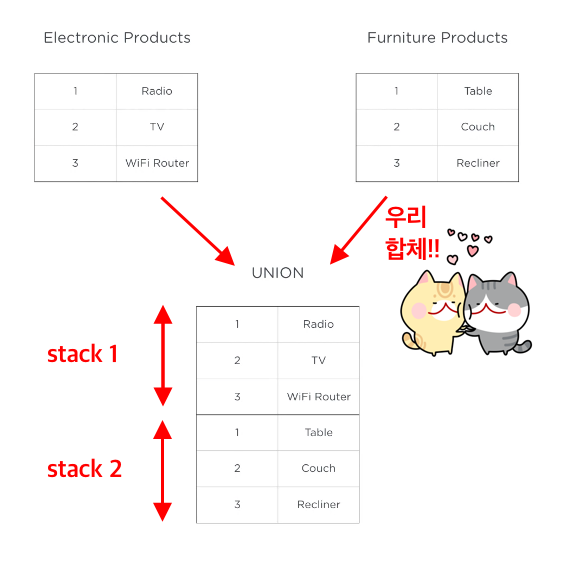
\includegraphics[width=0.8\linewidth]{images/part_5_notes_2.png}
    \end{center}

    \item has to have matching number of columns
    \item \textbf{Syntax:} \textit{query 1} UNION \textit{query 2}

    \bigskip

    \underline{\textbf{Example:}}

    \bigskip

    \begin{lstlisting}[language=SQL]
    SELECT MakeID, MakeName FROM Make UNION SELECT ForeignMakeID, MakeName FROM ForeignMake;
    \end{lstlisting}

    \bigskip

    \begin{center}
    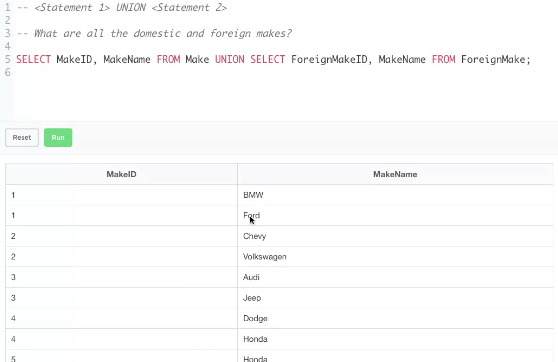
\includegraphics[width=0.8\linewidth]{images/part_5_notes_1.png}
    \end{center}

    \bigskip

    \underline{\textbf{Example 2:}}

    \bigskip

    \begin{lstlisting}[language=SQL]
    SELECT MakeID, MakeName FROM Make
        WHERE MakeName < "D"
    UNION
    SELECT ForeignMakeID, MakeName FROM ForeignMake
        WHERE MakeName < "D"
        ORDER BY MakeName;
    \end{lstlisting}

\end{itemize}

\bigskip

\section{Union All Operations}

\bigskip

\begin{itemize}
    \item Is the same as union but does not eliminate duplicates
    \item \textbf{Syntax:} \textit{query 1} UNION ALL \textit{query 2}
\end{itemize}

\bigskip

\section{Intersect}

\bigskip

\begin{center}
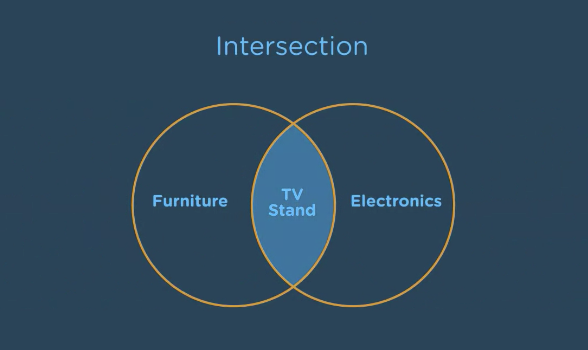
\includegraphics[width=0.8\linewidth]{images/part_5_notes_3.png}
\end{center}


\begin{itemize}
    \item Only returns results that exist in both
    \item Intersection is based on supplied columns
    \begin{itemize}
        \item multiple columns $\to$ intersection is based on intersecting values in those columns
    \end{itemize}
    \item \textbf{Syntax:} \textit{query 1} INTERSECT \textit{query 2}

    \bigskip

    \underline{\textbf{Example:}}

    \bigskip

    \begin{lstlisting}[language=SQL]
    SELECT MakeName FROM Make
        INTERSET
    SELECT MakeName FROM  ForeignMake ORDER BY MakeName DESC;
    \end{lstlisting}

    \bigskip

    \begin{center}
    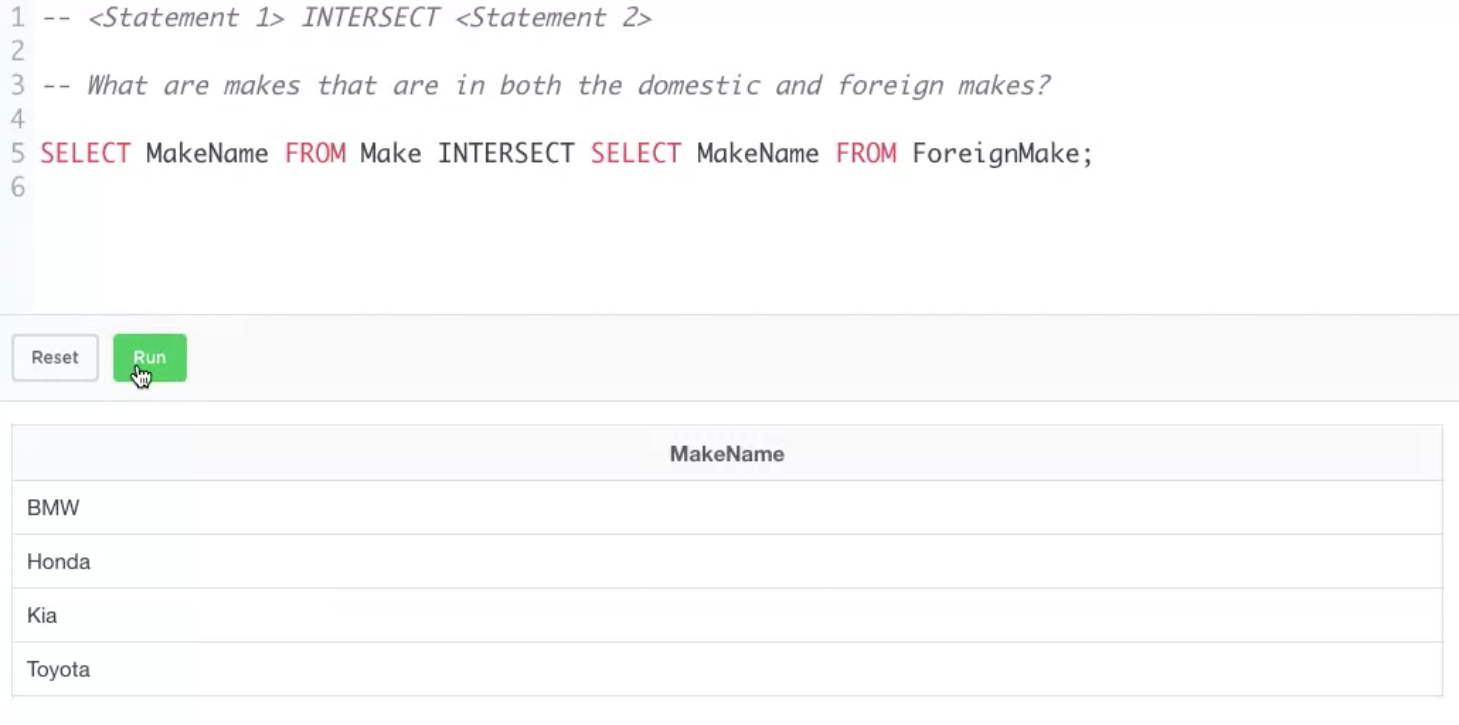
\includegraphics[width=\linewidth]{images/part_5_notes_4.png}
    \end{center}

    \bigskip

    \underline{\textbf{Example 2:}}

    \bigskip

    \begin{lstlisting}[language=SQL]
    SELECT MakeID MakeName FROM Make
        INTERSET
    SELECT ForeignMakeID, MakeName FROM  ForeignMake ORDER BY MakeName DESC; // <- Returns empty result
    \end{lstlisting}

    \begin{center}
    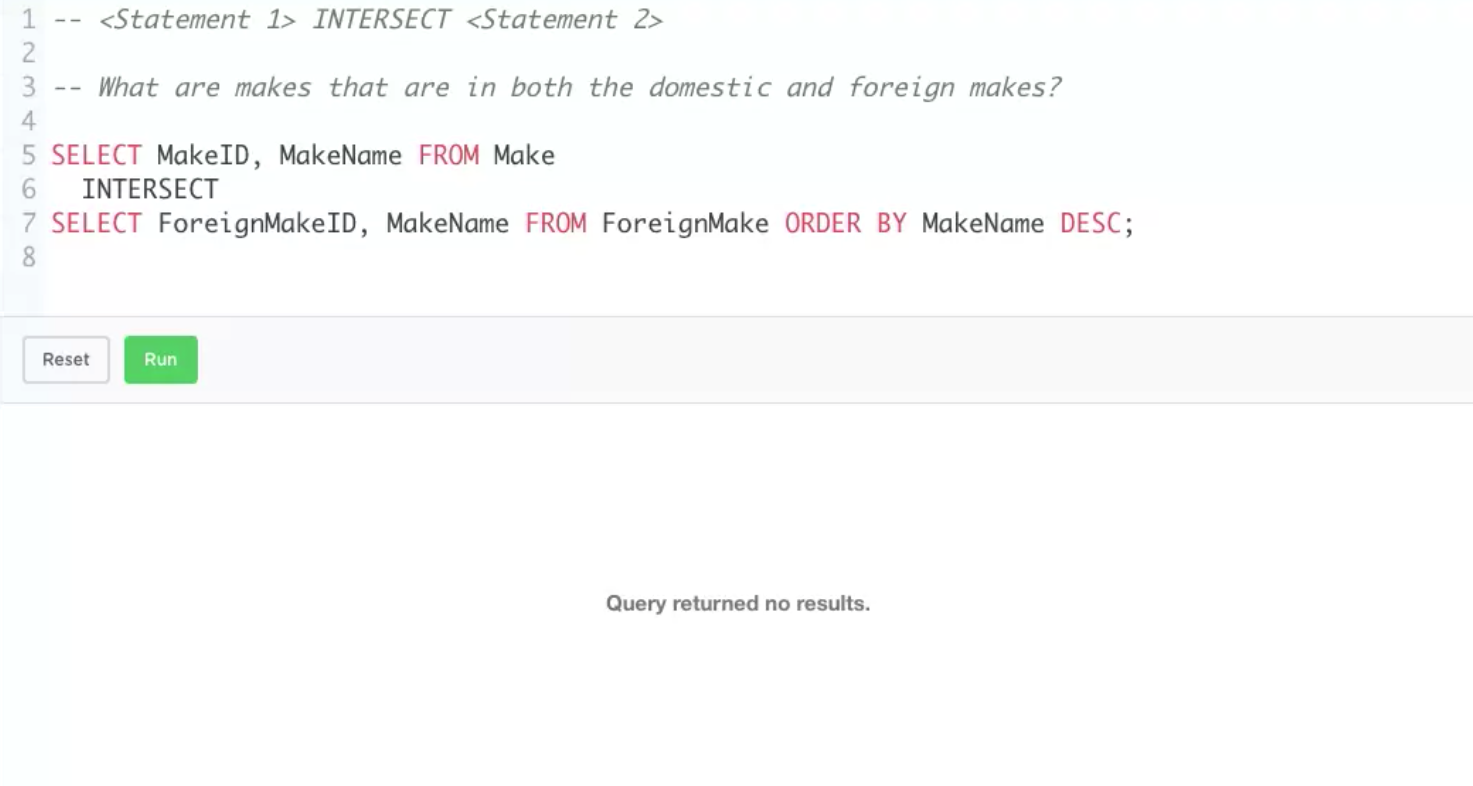
\includegraphics[width=\linewidth]{images/part_5_notes_5.png}
    \end{center}
\end{itemize}

\bigskip

\section{Except Operations}

\bigskip

\begin{center}
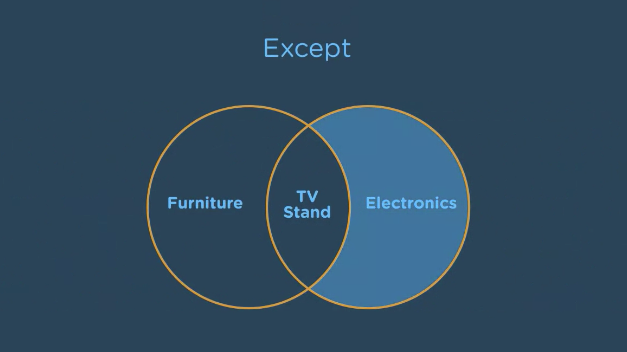
\includegraphics[width=0.8\linewidth]{images/part_5_notes_6.png}
\end{center}


\begin{itemize}
    \item \textbf{Syntax:} \textit{Query 1} EXCEPT \textit{Query 2}
    \item SQL accounts for all columns considered
    \item Except uses the same format as INTERSET but outputs only the records
    that are not in the latter table

    \bigskip

    \underline{\textbf{Example:}}

    \bigskip

    \begin{lstlisting}[language=SQL]
    SELECT ForeignMakeID, MakeName FROM ForeignMake EXCEPT SELECT MakeID, MakeName FROM Make; // shows only forien made goods
    \end{lstlisting}
\end{itemize}


\end{document}